\documentclass[11pt, letterpaper]{article}


% ---------------------------------------------------------
% Commands
\usepackage[utf8]{inputenc}
\usepackage{graphicx}
\usepackage{hyperref}
\usepackage{cite}
\usepackage{vmargin}
\usepackage{lipsum}
\usepackage{amsmath}
\usepackage{enumerate}
\usepackage{tcolorbox}


\setmargins{2.5cm}                 % margen izquierdo
{1.5cm}                            % margen superior
{16.5cm}                           % anchura del texto
{23.42cm}                          % altura del texto
{10pt}                             % altura de los encabezados
{1cm}                              % espacio entre el texto y los encabezados
{0pt}                              % altura del pie de página
{2cm}                              % espacio entre el texto y el pie de página


% \hyphenation{}


% \hypersetup{colorlinks,%
%   citecolor=blue,%s
%   filecolor=blue,%
%   linkcolor=blue,%
%   urlcolor=blue%
% }


% COMMANDS


% requires \usepackage{tcolorbox}
\newcounter{myboxcounter}
\newtcolorbox[auto counter, number within=section]{issue-box}[1][] {
   colback=red!10,
   colframe=red!80,
   fonttitle=\bfseries,
   title=Issue/Question \thetcbcounter: #1
}






% ---------------------------------------------------------
\title{\textbf{Report: Exploring The Regulation Image Space}}


% ---------------------------------------------------------


\date{}
\author{}


\newcommand{\vecsym}[1]{\boldsymbol{#1}}




% ---------------------------------------------------------
% opening
\begin{document}


\maketitle


% ---------------------------------------------------------
\section{Regulation Image Space}


The regulation process, in all its complexity, ultimately affects metabolism by controlling the flux in the network.
Regulation just adds extra constraints over a Minimally Constrained Network, $GEM^{0}$ (the supper index refers to the number of added constraints).
For a given regulatory state, there corresponds a set of constraints and a space of possible flux configurations.
If we consider all possible constraints applicable over a given $GEM^{0}$, we are then exploring all possible effects of regulation over such a network.
This space of constraints, in the current interpretation, is what we call the Regulation Image Space.


One aspect of this control is the limiting of the feasible flux range.
A physiological rationale that can explain such regulation is the control of enzyme abundances.
Such control does not necessarily set the flux of a reaction, which depends on other processes such as inhibition or reactant concentrations.
However, the quantity of enzymes does set an upper limit for a given flux.
In the case of a knockout, this limit is extreme, and the flux is actually defined.
Given that we know more about the structure of metabolic flux space than regulation states, it is tempting to explore the connection between them and try to discover general limitations or patterns in cellular regulation.


% ---------------------------------------------------------
\section{Hit and Down Monte Carlos}


% ---------------------------------------------------------
\subsection{Generate \texorpdfstring{$\vecsym{B^{ko}}$}{Bth} ensemble}


One approach for exploring the Regulation Image Space is using a Monte Carlo.
We procede as follow:


\begin{enumerate}[i]


   \item setup flux targets
   \label{setup flux targets}


   We will operate over the free variables of the system (free fluxes).
   Additionally, we want to operate just over the internal fluxes.
   We will not modify (add new constraints to) any property related with: the exchange fluxes, the biomass rate, not other non enzymatic reactions (ex: ATP maintenance).
   At the end we will have a vector of flux targets that enumerate the dimensions of the Regulation Image Space.
   We call this vector $\vecsym{f}$.


   \item setup Minimally Constrained Network
   \label{item:setup-Minimally-Constrained-Network}


   We set all flux bounds to be maximally unrestricted.
   This is our base model, which includes only the constant constraints.
   For instance, it will constraint the system to be coherent with the medium setup we are exploring.
   This network must be feasible (see step \ref{item:test-feasibility}).


   \item random downregulation
   \label{item:random-downregulation}


   We randomly select a reaction in $\vecsym{f}$ and modify it according to a downregulation strategy.
   This selection can be with or without replacement, depending on the chosen strategy.
   For instance, a knockout sets both reaction bounds to zero, so repeating a flux has no meaning.
   We assume these downregulations can be described by a vector $\vecsym{c}$, which we call a downvector.
   This will produce a new model $GEM^{d}$ (where $d$ is the number of added downregulations in $\vecsym{c}$).


   \item test feasibility
   \label{item:test-feasibility}


   We will explore the Regulation Image Space restricted to the region capable of producing biomass.
   For that, we perform $FBA$ and test if the optimal biomass is larger than a threshold, $z_{op} > z_{th}$.


   \item unfeasible downvector


   % TODO: check grammar
   We are adding more and more downregulations to the initial Minimally Constrained Network.
   Inevitably, as the number of downregulations grows ($d \gg 0$), this will lead to unfeasibility, $z_{op} < z_{th}$.
   We call it an unfeasible downvector $\vecsym{b^{ko}}$ or kovector.


   \item check duplication
  
   If we still have a feasible downvector, we jump to \ref{item:random-downregulation}.
   Otherwise, we will check if the downvector was produced before.
   We will consider downregulation strategies that produce the same network $GEM^{d}$ for all combinations of $\vecsym{b^{ko}_i}$.
   That is, $\vecsym{b^{ko}_i}$ order has no metabolic significance.
   $\vecsym{b^{ko}_i}$ can be viewed as a set, not a vector.
   For the other steps we will still attach to the vector definition because the last added downregulation is relevant as the frontier between feasibility and unfeasability.
   But for 'identity' we will use the set which elements are equal to the elements of $\vecsym{b^{ko}_i}$.
   So, if a previous kovector was produced with the same elements, we jump to \ref{item:reset-trajectory}.
   Otherwise we jump to \ref{item:record-kovectors}.
  
   \item record kovectors
   \label{item:record-kovectors}
  
   We will keep track of all produced non-duplicated unfeasible downvectors,
   $\vecsym{b^{ko}_i}$.
   This will produce an ensemble $\vecsym{B^{ko}}$ of unfeasible downvectors.
   You can see $\vecsym{B^{ko}}$ as a matrix where each row is a downvector.
  
   \item reset trajectory
   \label{item:reset-trajectory}


   For a reset, we remove a random number of elements from $\vecsym{b^{ko}_i}$.
   The removal should include at least the last added downregulation.
   This ensures that the resulting downvector is a feasible one.
   This is equivalent to 'moving' back a number of steps in the simulation.
   Also, it is important that removing all downregulations has a nonzero probability.
   That is, eventually, we will have restarts from the base model.


   After the reset, we jump again to \ref{item:random-downregulation}.


\end{enumerate}


% ---------------------------------------------------------
\subsection{Generate \texorpdfstring{$\vecsym{B^{fea}}$}{Bth} ensemble}


We can use $\vecsym{B^{ko}}$ as the basis for generating a set of feasible downvectors, feavectors $\vecsym{b^{fea}}$.
For the sampling we proceed as follow:


\begin{enumerate}[i]
  
   \item select a kovector from $\vecsym{B^{ko}}$.
       \label{item:select-kovector}
      
       This step can be exhaustive, partial, or random.
      
   \item generate feavectors from $\vecsym{b^{ko}_i}$.
       \label{item:select-feavector}
      
       Produce feavectors $\vecsym{b^{fea}_i}$ by combining elements of $\vecsym{b^{ko}_i}$.
       The selection cannot include the last element of $\vecsym{b^{ko}_i}$ to ensure feasibility.
       Starting from a kovector, we are sure that we are generating feasible downsets.
       There exists a combinatorial explosion associated with the production of possible feasets.
       By reducing the exploration to subsets of $\vecsym{B^{ko}}$, we reduce the impact of such an explosion.
      
       Also, the number of feavectors produced from the same $\vecsym{b^{ko}_i}$ can be tuned.
       This way, we can control the level of 'resolution' of the sampling but still claim we have a homogeneously distributed sample set. 


   \item produce ensemble
  
   By collecting all feasible downvectors, we produce an ensemble $\vecsym{B^{fea}}$.


\end{enumerate}




% ---------------------------------------------------------
\section{Results}


We can now study the properties of the networks produced by the downregulation process.
We will show results of EColi IJR904 genome-scale network with glucose as the only carbon source.
We will be performing total knockouts, but the same process can be applied to partial downregulations.




% ---------------------------------------------------------
\subsection{Monte Carlo equilibrium}


One way to evaluate if the exploration of the space is statistically significant, is to track derived distributions' evolution as we sample the space.
If it converges to a stable distribution, we can say that we have reached an equilibrium.
Figure \ref{fig:feaset.len.hist} show the histogram of the number of elements in the feavectors.
Although the distribution is stable in time, its shape is odd.


\begin{issue-box}[]
   \label{issue:feaset.len.hist}
   There is no clear explanation for the abrupt cut of the right tail of the distribution at fig \ref{fig:feaset.len.hist}.
   I will study this problem with the EColiCore network.
\end{issue-box}




\begin{figure}[h!]
   \centering
   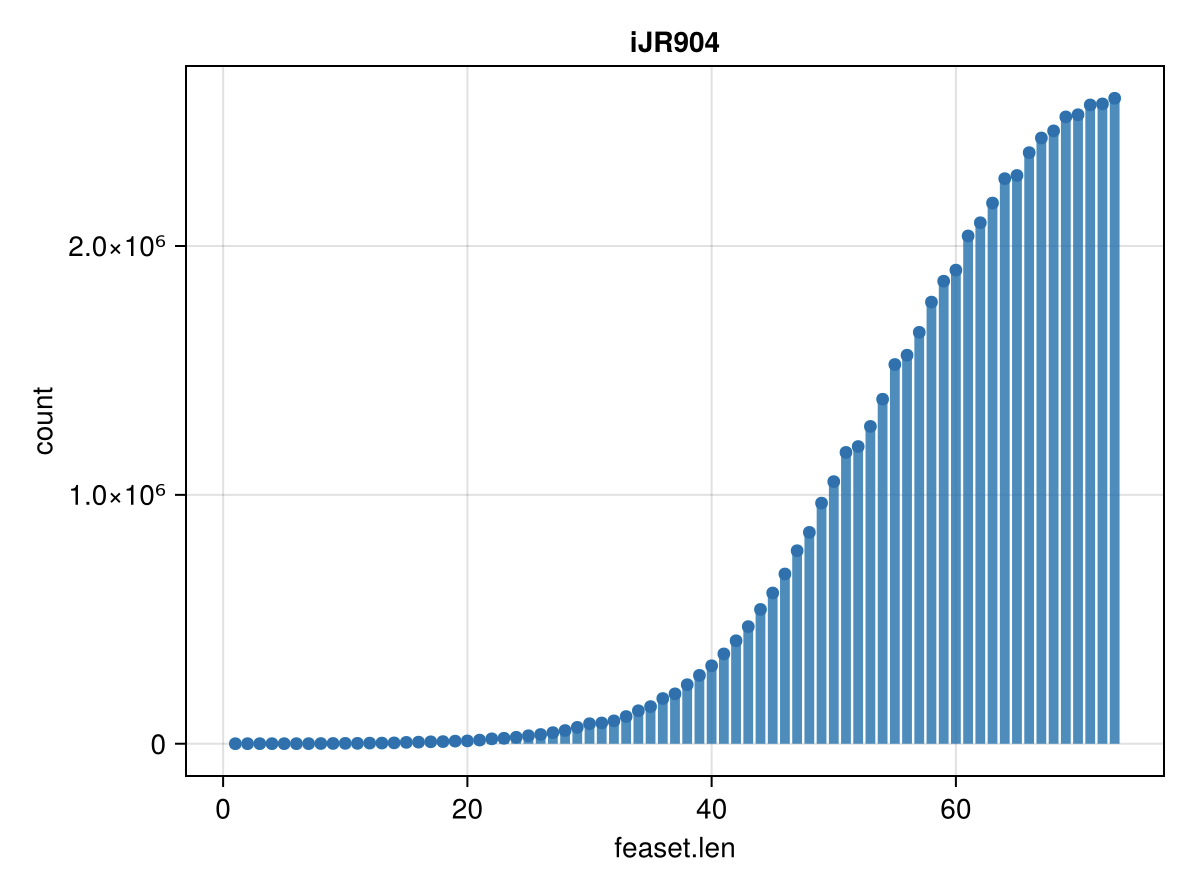
\includegraphics[width=0.5\textwidth]{images/feaset_len_hist.png}
   \caption{
       Histogram of the number of elements in the feavectors sampled from IJR904 derived Minimally Constrained Network.
   }   
   \label{fig:feaset.len.hist}
\end{figure}




% ---------------------------------------------------------
\subsection{FBA}


Now that we have an ensemble of feasible but constrained networks, we can see if the constant constraints are sufficient for suggesting limitations for the regulation.
One first property of the networks we can try to study is the solutions of biomass optimizations.




\begin{issue-box}[]
   \label{issue:yield.hist.1}
   There are observations of yields more than 2x larger than the theoretical predictions (see fig \ref{fig:yield.hist} first panel).
   Possible explanations: i. Biomass composition variability ii. Mutants/strains with crazy new enzymes. iii. experimental error.
   I think the first one is more likely.
\end{issue-box}


\begin{issue-box}[]
   \label{issue:yield.hist.2}
   We do not have data for the low yield region.
   I'm working on it. Maybe anaerobic conditions.
\end{issue-box}


\begin{figure}[h!]
   \centering
   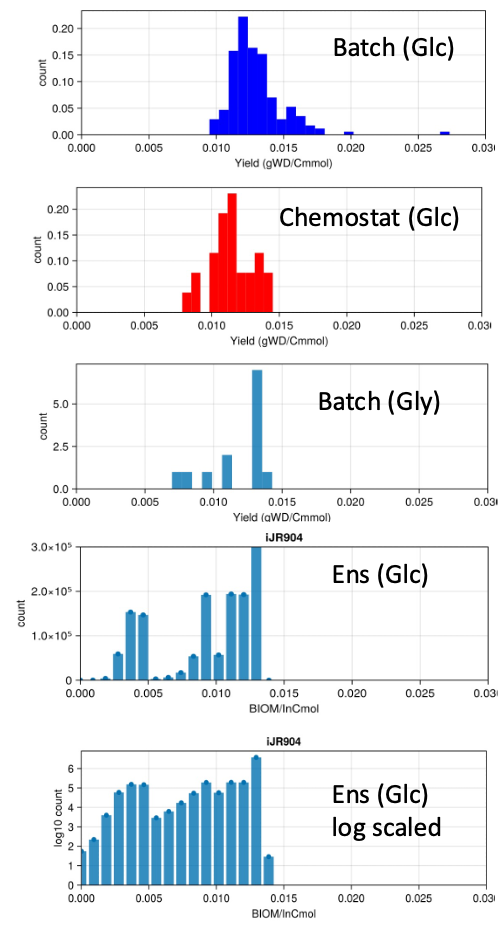
\includegraphics[width=0.5\textwidth]{images/yield_hist.png}
   \caption{
       Histogram of the biomass yield for the sampled feavectors from IJR904 derived Minimally Constrained Network.
   }
   \label{fig:yield.hist}
\end{figure}


\begin{issue-box}[]
   \label{issue:yield.ex_o2.corr}
   You can see that in \ref{fig:yield.ex_o2.corr} there are lineal traces.
   How is that possible? Each point is in theory a different $\vecsym{b^{fea}}$ defining a different $GEM^{d}$.
   How knocking a random subset of reactions leads to linear relationships.
   I will study this problem with the EColiCore network.
\end{issue-box}




\begin{figure}[h!]
   \centering
   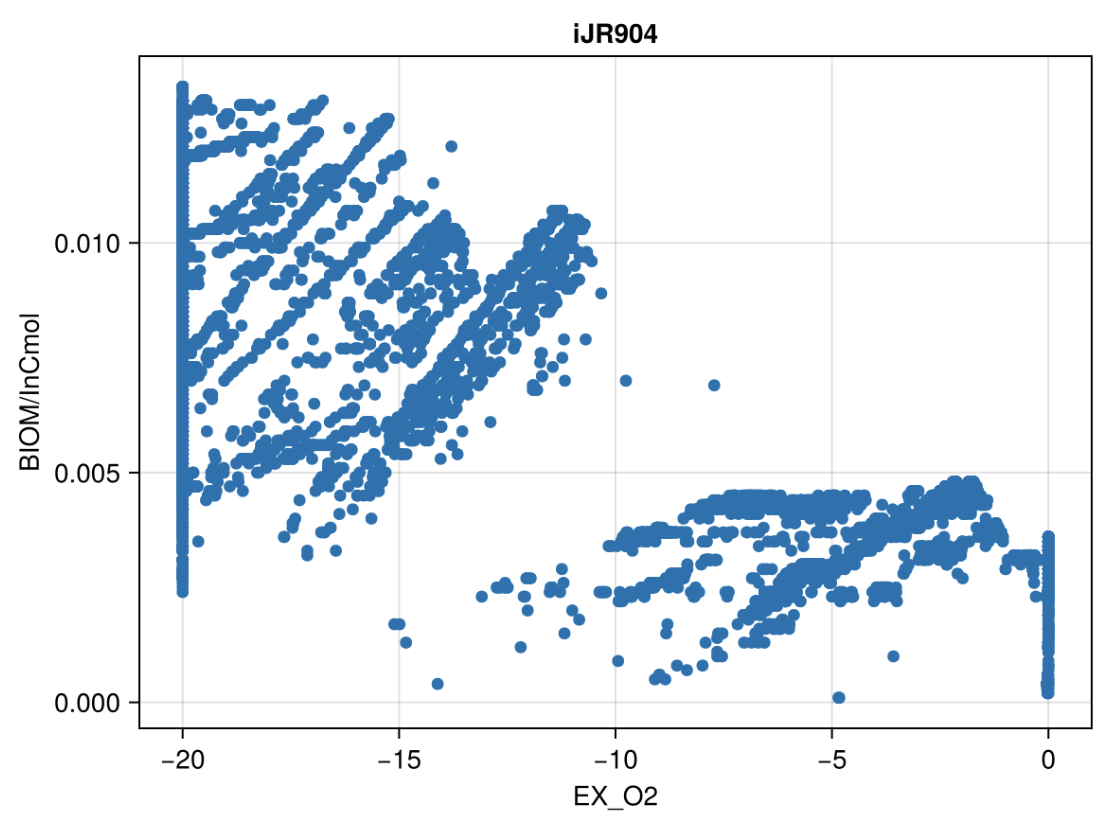
\includegraphics[width=0.5\textwidth]{images/yield_ex_o2_corr.png}
   \caption{
       Correlation of the biomass yield vs oxygen exchange from IJR904 derived Minimally Constrained Network.
   }
   \label{fig:yield.ex_o2.corr}
\end{figure}




\begin{issue-box}[]
   \label{issue:yield.ex_glc.corr}
   At fig \ref{fig:yield.ex_glc.corr} the issue is: why is the glucose not always totally consumed?
   The model has glucose as the sole carbon source.
   If we are maximizing the biomass, the model is feasible.
   How and why is the glucose not consumed?
   The biomass is not bounded and there are no internal constraints as enzymatic costs.
   The glucose intake is bound to 10.
   Maybe numerical problems.
   I will study this problem with the EColiCore network.
\end{issue-box}


\begin{figure}[h!]
   \centering
   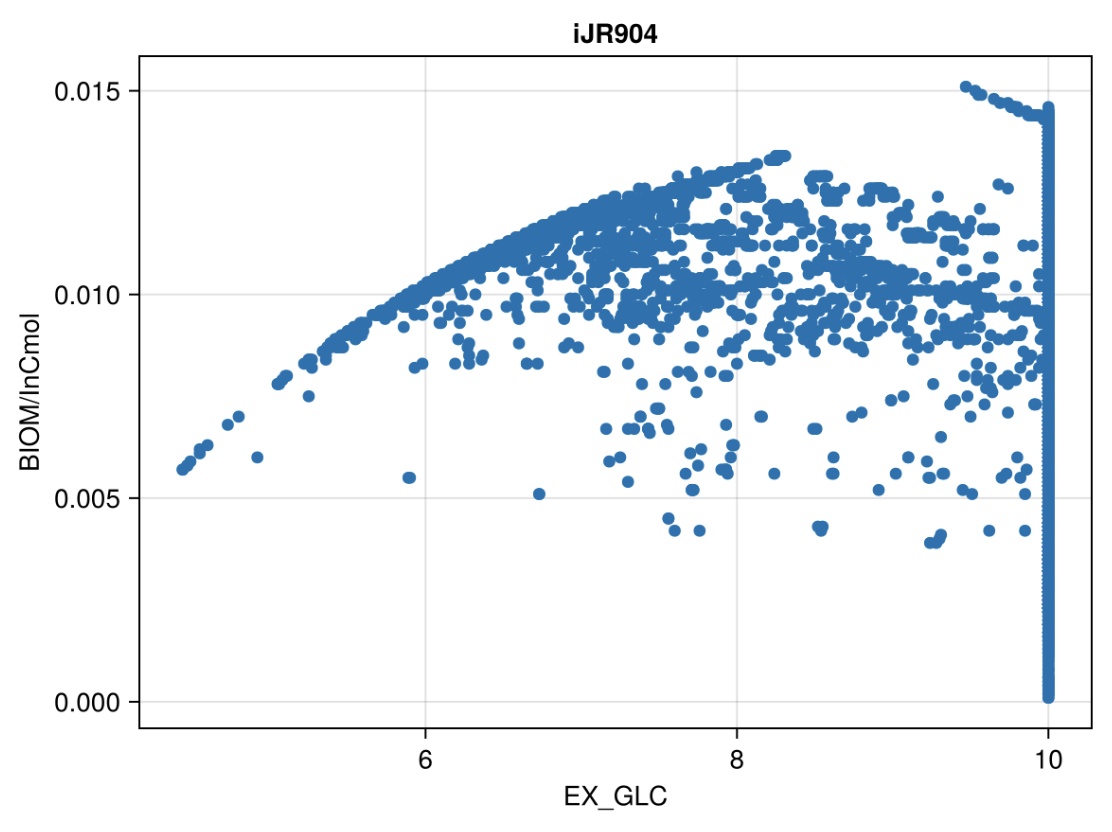
\includegraphics[width=0.5\textwidth]{images/yield_ex_glc_corr.png}
   \caption{
       Correlation of the biomass yield vs glucose exchange from IJR904 derived Minimally Constrained Network.
   }
   \label{fig:yield.ex_glc.corr}
\end{figure}


% ---------------------------------------------------------
\section{Conclusions}


The simulations can be carried out with full genome scale networks.
There are some results that I do not understand.




\bibliographystyle{plain}
\bibliography{main}
  
\end{document}

